\documentclass[12pt, twoside]{article}
\usepackage[letterpaper, margin=1in, headsep=0.5in]{geometry}
\usepackage[english]{babel}
\usepackage[utf8]{inputenc}
\usepackage{amsmath}
\usepackage{amsfonts}
\usepackage{amssymb}
\usepackage{tikz}
\usetikzlibrary{quotes, angles}
\usepackage{venndiagram}
\usepackage{multicol}

\usepackage{fancyhdr}
\pagestyle{fancy}
\fancyhf{}
\renewcommand{\headrulewidth}{0pt} % disable the underline of the header
%\renewcommand{\baselinestretch}{1.5}

\fancyhead[RE]{\thepage}
\fancyhead[RO]{\thepage \\ Name: \hspace{3cm}}
\fancyhead[L]{BECA / Dr. Huson / IB Math\\* 7 November 2019}


\begin{document}
\subsubsection*{2.16 Pop Quiz: Descriptive statistics introduction}

\begin{enumerate}

  \item Write down the topic of your exploration paper. Start with the phrase, ``The aim of my paper is ...''  \vspace{3cm}
  
  \item For homework, you read an exploration paper written by a BECA student last year titled, \emph{Subway Linear Regression}. Where did the author collect his data?  \vspace{1cm}
  
  \item A box contains 100 cards. Each card has a number between one and six written on it. The following table shows the frequencies for each number.
  
  \begin{tabular}{|l|r|r|r|r|r|r|}
    \hline
    Number & 1 & 2 & 3 & 4 & 5 & 6\\ 
    \hline 
    Frequency & 26 & 10 & 20 & $k$ & 29 & 11\\ 
    \hline 
    \end{tabular}

  \begin{enumerate}
    \item Calculate the value of $k$. \hfill [3 marks] \vspace{3cm}
    \item Find
    \begin{enumerate}
      \item the median; \hfill [2 marks] \vspace{3cm}
      \item the interquartile range. \hfill [3 marks] \vspace{3cm}
    \end{enumerate}
  \end{enumerate}

\newpage

  \item The following box-and-whisker plot represents the examination scores of a group of students.\\
  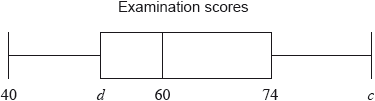
\includegraphics[width=9cm]{2-16exam-scores-box-plot.png}
  \begin{enumerate}
    \item Write down the median score. \hfill [1 marks]\\[1.5cm]
    The range of the scores is 52 marks, and the interquartile range is 19 marks.
    \item Find the value of
    \begin{enumerate}
      \item $c$; \hfill [2 marks] \vspace{2cm}
      \item $d$. \hfill [2 marks] \vspace{2cm}
    \end{enumerate}
  \end{enumerate}

  \item The scores of 30 students taking an IB Paper 2 are shown in the frequency table below.
    
    \begin{tabular}{|l|c|c|c|c|}
      \hline
      Mark ($x$) & $10 \leq x < 30$ & $30 \leq x < 50$ & $50 \leq x < 70$ & $70 \leq x < 90$\\ 
      \hline 
      Frequency & 8 & 12 & 7 & 3\\ 
      \hline 
      \end{tabular}

    \begin{enumerate}
      \item Write down the modal class.  \hfill [1 mark]  \vspace{2cm}
      \item Estimate the mean score $\overline{x}$. \hfill [3 marks] \vspace{2cm}
      \item Estimate the standard deviation of the scores, $\sigma$.  \hfill [3 marks] \vspace{1cm}
    \end{enumerate}

\end{enumerate}
\end{document}
